\chapter{Mise en place d'une solution \alinotp{}}
\label{section:linotp}

\section{Principe des \etranger{One-Time Passwords} (OTP)}

\paragraph{}
Les \etranger{One-Time Passwords}, aussi appelés OTP, sont des mots de passe générés à un instant donné, valides pendant une courte durée et utilisables une seule fois.
La génération s'effectue grâce à des matériels adaptés, comme les tokens (\cffigure{linotp:token}) ou même des smartphones.

\begin{figure}
	\centering
	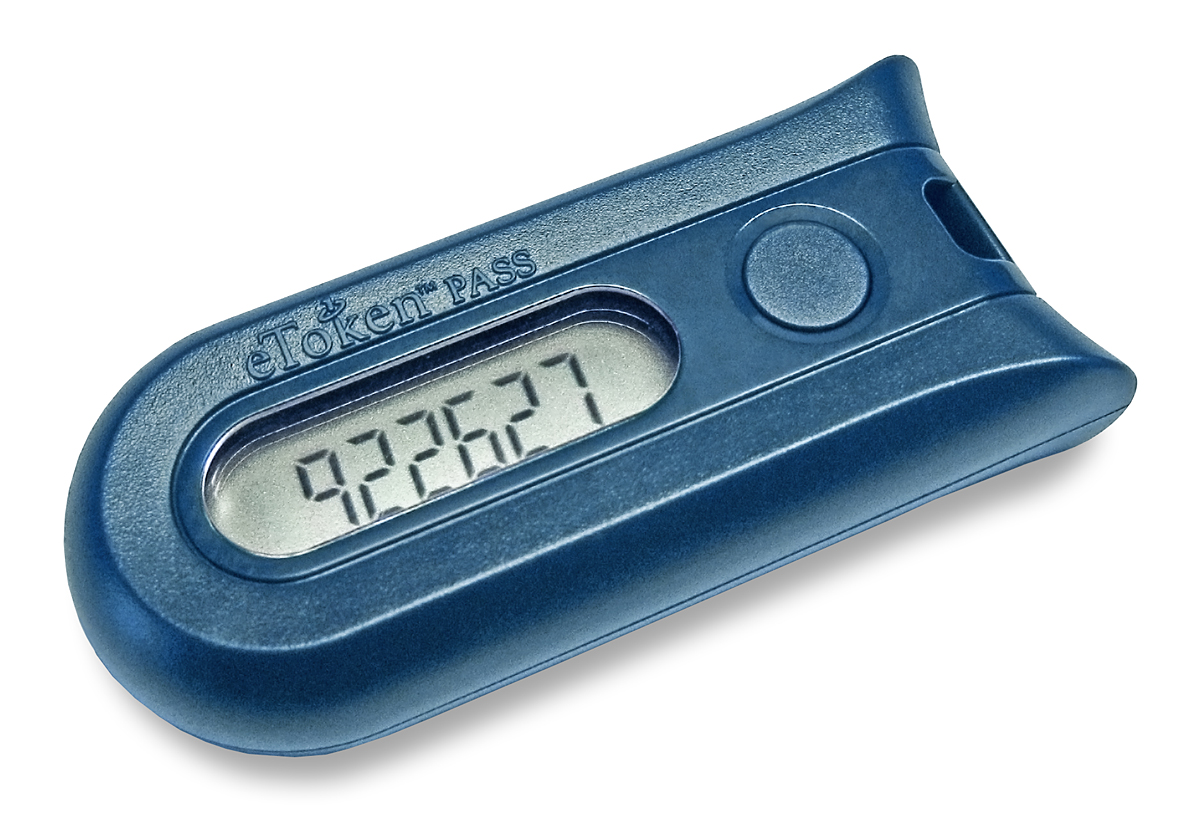
\includegraphics[width=6cm]{linotp/etoken_pass}
	\caption{Token Aladdin eToken-PASS}
	\label{figure:linotp:token}
\end{figure}

\paragraph{}
En pratique, l'utilisateur final s'authentifie en précisant son identifiant, son PIN -- qui correspond à un mot de passe statique qu'il doit mémoriser -- et l'OTP obtenu grâce au matériel.
C'est en ce sens qu'on peut parler de système à deux facteurs d'authentification (\etranger{two-factor authentication}) car on se base sur quelque chose que l'on connaît -- le PIN -- et quelque chose que l'on possède -- le token ou le smartphone.

\paragraph{}
Ainsi, l'OTP permet de résoudre un certain nombre de problèmes inhérents à l'utilisation de mots de passe statiques classiques :

\begin{itemize}
	\item on n'est plus soumis aux limites du facteur humain, qui implique souvent des compromis sur la complexité du mot de passe, et l'irrégularité de son changement ;
	\item en particulier les attaques par dictionnaire deviennent inefficaces ;
	\item les attaques par brute-force sont également limitées car elles ne peuvent plus se baser que sur des essais aléatoires dans un grand espace de clés ;
	\item la récupération silencieuse du mot de passe (via l'écoute réseau, l'installation d'un mouchard, ou l'ingénierie sociale) ne suffit plus à s'authentifier.
\end{itemize}

\paragraph{}
Par ailleurs, une méthode de génération d'OTP se base sur la synchronisation temporelle : les tokens et le serveur d'authentification OTP sont réglés à la même heure.
De plus, pour chaque token est définie une clé secrète que l'on enregistre dans la base du serveur.
C'est la combinaison de ces deux paramètres qui permet une génération et une validation des OTP.


\section{Contexte de la mission}

\paragraph{}
Au courant de l'année 2010, la Commission nationale de l'informatique et des libertés\footnote{La CNIL est une autorité administrative indépendante française. Elle est chargée de veiller à ce que l'informatique soit au service du citoyen et qu'elle ne porte atteinte ni à l'identité humaine, ni aux droits de l'homme, ni à la vie privée, ni aux libertés individuelles ou publiques.~\cite{cnil}} (CNIL) décide d'ouvrir son portail \aintranet{} confidentiel sur l'\ainternet{} pour certains de ses utilisateurs : les commissaires.
Au nombre d'une vingtaine, ceux-ci ont besoin d'accéder au contenu du site web à l'extérieur de leur lieu de travail -- à la maison par exemple.

\paragraph{}
La CNIL avait déjà fait appel aux prestations de \asmile{} pour bénéficier d'un support ponctuel sur des développements \atypo{}\footnote{\atypo{} est un système de gestion de contenu libre écrit en PHP. Fourni de base avec un certain nombre de fonctionnalités, il peut être étendu de manière impressionnante grâce à un puissant moteur de plugins. Une console d'administration permet aux auteurs et aux administrateurs de gérer facilement le contenu du site web.}, le système de gestion de contenu utilisé pour le portail.
C'est pour cela qu'elle a également choisi \asmile{} pour mettre en place l'architecture permettant un tel accès depuis l'extérieur.

\paragraph{}
C'est la CNIL elle-même qui a choisi le type d'authentification à utiliser : les OTP.
\asmile{} a alors proposé fin 2010 l'utilisation d'une solution de la marque RSA, leader sur ce marché.
Pour des raisons qui sont restées inconnues -- le nombre de licences commandées était trop faible ? -- RSA n'a pas daigné répondre aux commandes de licences et de matériel réalisées par \asmile.

Le retard sur la mise en place de l'architecture a alors poussé \asmile{} à changer de solution pour se tourner vers une alternative open source : \alinotp{}.


\section{La solution \alinotp{}}

\paragraph{}
La solution \alinotp{} se place au centre du mécanisme d'authentification :

\begin{itemize}
	\item l'interface de connexion utilisateur du portail demande à \alinotp{} de valider ou non l'authentification ;
	\item \alinotp{} consulte une base de données des utilisateurs déjà existante (e.g. un LDAP) ;
	\item les informations concernant les matériels OTP sont stockées dans sa propre base de données.
\end{itemize}

\paragraph{}
D'un point de vue technique, \alinotp{} est un serveur écrit en langage Python, avec lequel on communique par de simples requêtes HTTP.
Il est donc possible de l'administrer via d'autres outils que ceux fournis dans la distribution.
On peut imaginer développer une interface web spécifique que l'on inclurait dans une section privilégiée d'un Intranet par exemple.

\paragraph{}
Par ailleurs, \alinotp{} se décline en deux éditions :

\begin{itemize}
	\item l'édition Community, libre et gratuite, qui propose des fonctions de base pour mettre en place une maquette ;
	\item l'édition Enterprise, pour laquelle il faut acheter des licences en fonction du nombre de tokens utilisés, propose un vraie solution pour des besoins d'entreprise, avec notamment le support LDAP, \aad{}, SQL ou encore \afreerad{}.
\end{itemize}

\paragraph{}
La \reffigure{linotp:linotp-archi} illustre l'architecture modulaire de \alinotp{}~2 tout en mettant en évidence les possibilités de la solution :

\begin{itemize}
	\item en rouge est représenté le c\oe ur de \alinotp{} -- le serveur ainsi que sa base de tokens stockée dans une base de données externe ;
	\item en vert, on retrouve les différentes interfaces de résolution des utilisateurs ;
	\item en jaune, les interfaces d'authentification seront contactées par les pro\-gram\-mes clients de la solution qui demanderont si un couple identifiant~/~mot de passe OTP est bien valide ;
	\item enfin, en bleu on retrouve les différentes interfaces qui permettent d'administrer \alinotp{}, que ce soit par le web ou en ligne de commande.
\end{itemize}

\begin{figure}
	\centering
	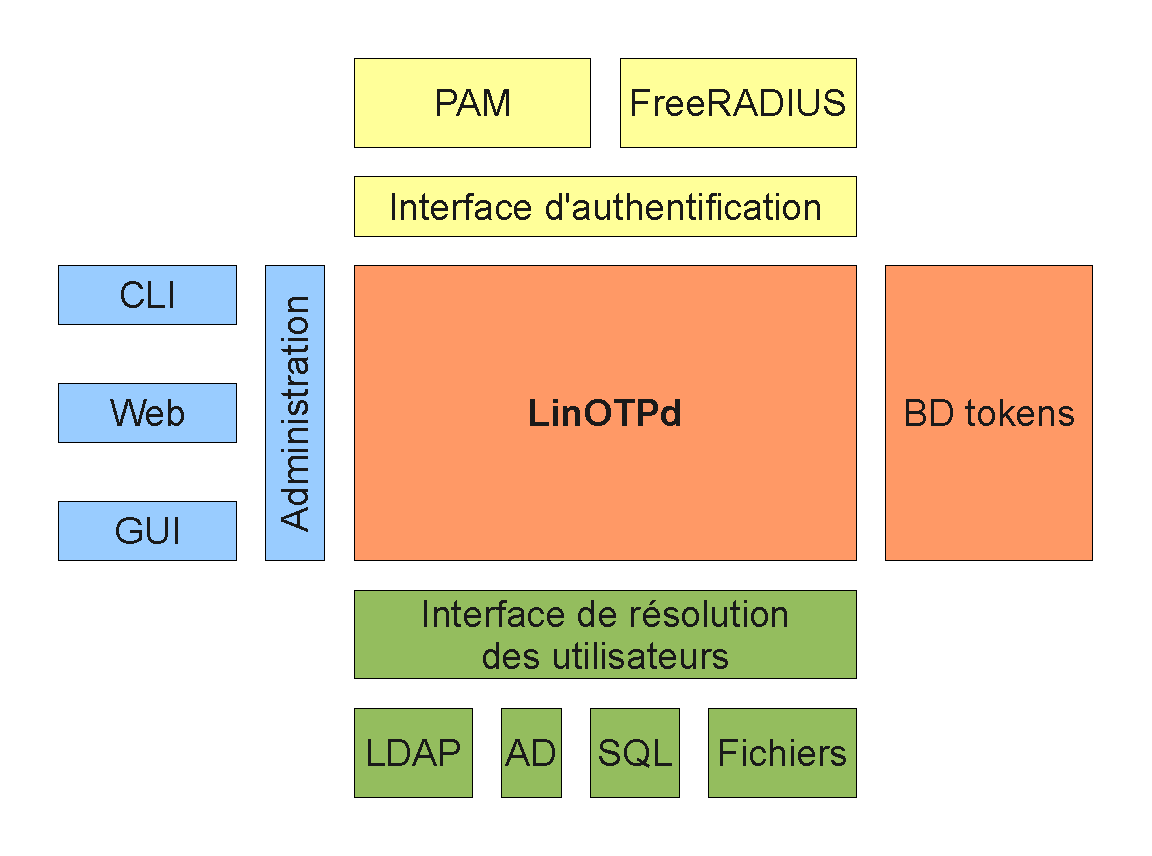
\includegraphics[width=10cm]{linotp/linotp-archi}
	\caption{Architecture modulaire de \alinotp{}~2}
	\label{figure:linotp:linotp-archi}
\end{figure}


\section{Ma démarche}

\paragraph{Mise en place d'un prototype}
C'est mon manager \apakou{} qui m'a confié la responsabilité de mettre en place la solution \alinotp{} chez notre client.

Après m'avoir présenté le contexte de la mission ainsi que le principe des OTP, il m'a demandé de mettre en place une première maquette fonctionnelle du système.
Les détails techniques de ce prototype seront décrits dans la \refsection{linotp:prototype}.

\paragraph{Présentation du prototype}
J'ai pu alors présenter ma maquette à deux reprises.

La première fois, je me suis rendu avec \asegir{}, le chef de projet de la mission, dans les bureaux de la \abugan.
En effet, ses développeurs sont responsables de la partie concernant l'adaptation du portail \atypo{} de la CNIL pour cette mission.
Grâce à ma démonstration du prototype, ils ont donc bien pu comprendre comment l'authentification OTP allait se dérouler pour les utilisateurs finaux.
Ils ont également pu obtenir les détails techniques concernant les flux de données que \atypo{} recevra de \alinotp{} et qu'ils devront traiter.

La seconde fois, nous nous sommes rendus, \apakou, \asegir{} et moi, dans les locaux du client pour faire valider mon travail par nos deux interlocuteurs : \ahbt, chef du service informatique de la CNIL, et \amimiette, un administrateur système.
Pour l'occasion, j'ai présenté un diaporama récapitulant le fonctionnement de la solution du point de vue de l'utilisateur final et décrivant techniquement via des diagrammes quelle allait être l'architecture à mettre en place, avec ses pré-requis.
J'ai pu terminer avec une démonstration du système via mon prototype.

\paragraph{Contact avec l'éditeur}
Une fois mon prototype validé, j'ai contacté directement l'éditeur \alse{} pour passer la commande de 30 tokens ainsi que des 30 licences \alinotp{} Enterprise correspondantes.
En effet, la version Enterprise est nécessaire du fait que les utilisateurs sont résolus depuis un annuaire \aad{} et que l'authentification doit se faire via un serveur \aradius.

J'en ai profité pour leur demander des conseils sur les différentes briques logicielles à utiliser sur l'architecture finale.
Par la suite, j'ai également pu leur faire de nombreux retours sur les problèmes que j'ai rencontré et sur la façon dont j'ai pu les contourner.
Cette échange donnant-donnant a été très bénéfique et présage un futur partenariat privilégié entre \asmile{} et \alse{}.

\paragraph{Mise en place de l'architecture finale}
Les détails techniques de l'architecture finale seront décrits dans la \refsection{linotp:archi-finale}.

J'ai commencé par mettre en place le système sur des environnements virtuels hébergés sur des serveurs de \asmile{}.
Cela m'a permis d'être rapidement confronté aux premiers problèmes et de les résoudre avant d'intervenir chez le client.

Une fois ma maquette jugée satisfaisante et répondant au besoin, j'ai pris rendez-vous avec le client pour mon intervention.
J'ai alors travaillé avec \amimiette{} qui m'a expliqué comment m'intégrer efficacement à leur infrastructure système existante.
Cette première intervention a duré deux jours.
En outre, j'ai pris des notes relatives à mon travail sur leurs serveurs au fur et à mesure afin de pouvoir par la suite rédiger une documentation technique complète.

Aussi, j'ai dû rapidement intervenir une seconde fois afin de corriger un premier bug découvert : l'authentification d'un utilisateur, bien qu'elle soit correcte, n'était pas considérée comme valide environ 1 fois sur 3.
J'ai pu rapidement cibler le problème qui provenait de la connectivité avec l'annuaire \aad.
J'en ai parlé avec \amimiette{} qui s'est rappelé avoir eu un problème similaire par le passé avec un précédent prestataire de \asmile : il s'agissait en fait d'une option de configuration LDAP à désactiver sur le serveur hébergeant ma solution \alinotp. 

Mon infrastructure OTP enfin fonctionnelle, \arolel{}, un développeur de la \abugan{}, a pu intervenir à son tour une journée pour adapter le portail \atypo{} au nouveau mode d'authentification.
Tout s'est bien passé mais il lui manquait des informations pour implémenter la fonctionnalité de déconnexion de l'utilisateur.

J'ai dû finalement intervenir une troisième fois seul pour adapter mon infrastructure à cette fonctionnalité, puis une quatrième et dernière fois avec \arolel{} pour tout finaliser et tester fonctionnellement le système.

\paragraph{Retour d'expérience et capitalisation}
Cette expérience était une première chez \asmile{} en terme de mise en place d'authentification OTP et je suis heureux d'en avoir été l'un des acteurs.
Elle a alors fait l'objet d'un article dédié dont je suis l'auteur sur le blog de \asmile{}\footnote{Certaines parties de cette section sur mon expérience avec \alinotp{} reprennent mot pour mot mon article sur le blog de \asmile{}. Comme j'en suis l'auteur, cela ne peut en aucun cas faire l'objet d'une accusation de plagiat.}~\cite{blog}.

Par ailleurs, la capitalisation s'est concrétisée côté \asmile{} par une page de documentation sur le wiki technique et côté CNIL par une documentation technique et une documentation utilisateur.


\section{Architecture du prototype}
\label{section:linotp:prototype}

\paragraph{Environnement}
Mon prototype a été mis en place sur une machine virtuelle VirtualBox.
Ce type de machine virtuelle a l'avantage d'être portable et d'être facilement copié ou déplacé sur plusieurs ordinateurs différents.
C'était donc le format idéal pour effectuer les deux présentations du prototype chez \asmile{} et chez le client.

\begin{figure}
	\centering
	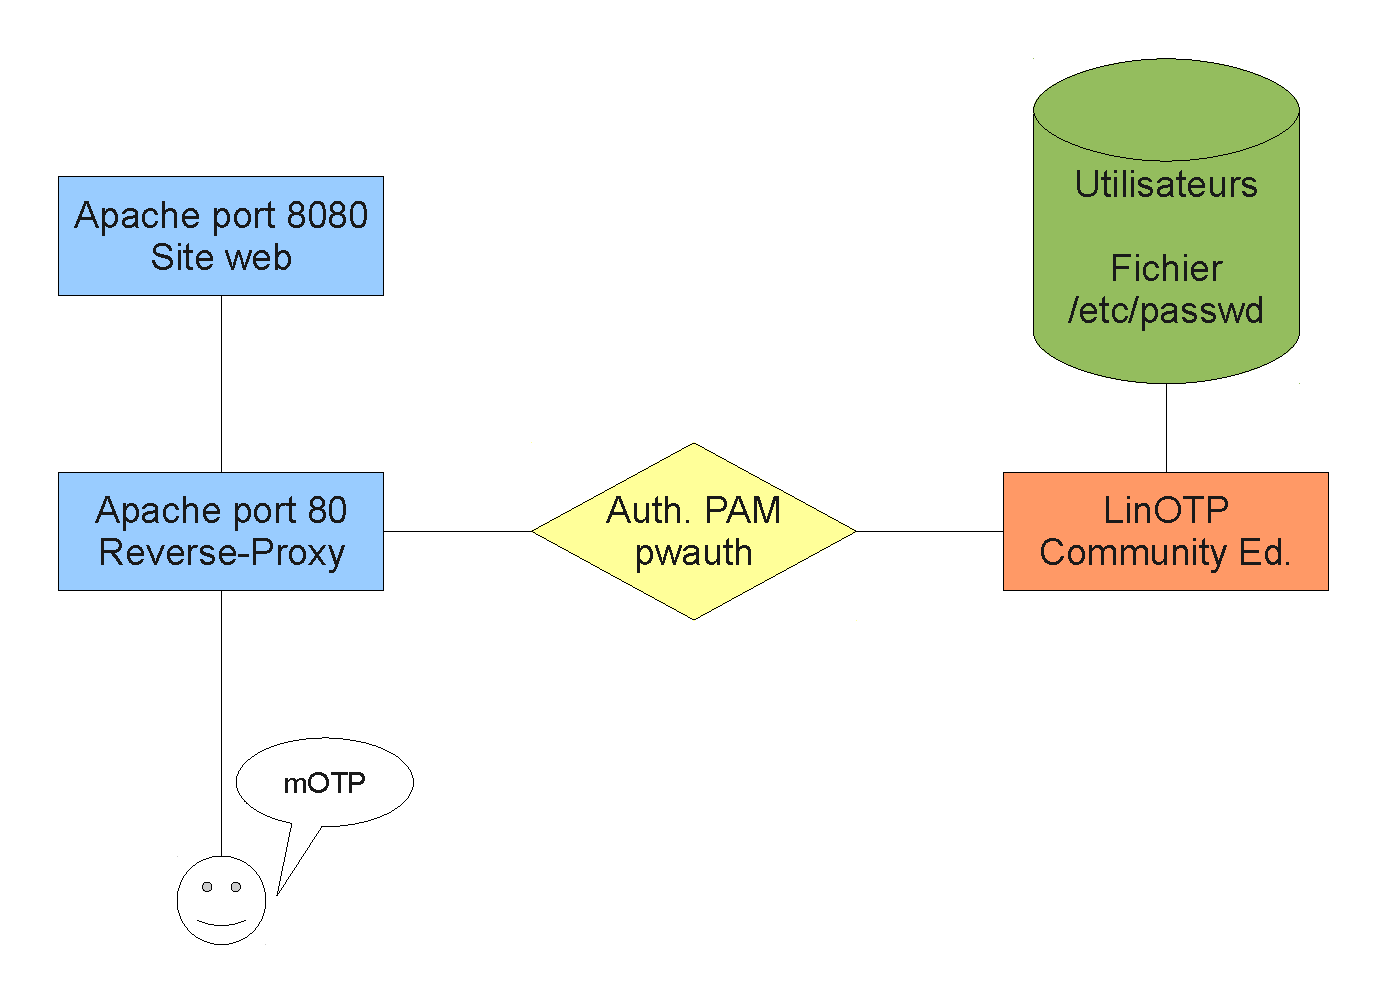
\includegraphics[width=12cm]{linotp/archi-proto}
	\caption{Architecture du prototype \alinotp}
	\label{figure:linotp:archi-proto}
\end{figure}

\paragraph{Architecture}
L'architecture est illustrée en \reffigure{linotp:archi-proto}.
Elle a été mise en place sur un système \alinux{} Debian.

Le portail \aintranet{} \atypo{} est symbolisé par une simple page web hébergée sur un serveur HTTP Apache.
Elle est accessible depuis l'intérieur du réseau \aintranet{} sur le port 8080.
Ce port n'est pas accessible depuis l'extérieur.

Au contraire, le port 80 du serveur Apache peut être contacté depuis \ainternet.
Un \arp{} est alors configuré : l'intérêt est de faire passer l'utilisateur par intermédiaire de ce serveur HTTP pour accéder à la page accessible en interne sur le port 8080.
Celle-ci reste donc toujours isolée de l'extérieur.

Une authentification HTTP Basic\footnote{Dans le cadre d'une transaction HTTP, l'authentification Basic est une méthode permettant de fournir un identifiant et un mot de passe lors d'une requête. Ce couple est fourni via les en-têtes de la requête HTTP.~\cite{httpbasic}} est mise en place sur ce \arp{}.
Quand l'utilisateur a entré son identifiant et son mot de passe issu d'un OTP, le module Apache \amodpam{} prend le relais et réalise une authentification PAM\footnote{Pluggable Authentication Modules (en abrégé PAM) est un mécanisme permettant d'intégrer différents schémas d'authentification de bas niveau dans une API de haut niveau, permettant de ce fait de rendre indépendants du schéma les logiciels réclamant une authentification. PAM est une création de Sun Microsystems et est supporté en 2006 sur les architectures Solaris, \alinux, FreeBSD, NetBSD, AIX et HP-UX.~\cite{pam}}.
Ainsi, on filtre les utilisateurs de façon à ce que seuls ceux qui ont été acceptés par \alinotp{} puissent rentrer.

En effet, un serveur \alinotp{} Community Edition est mis en place, car nous ne disposions pas encore des licences pour la version Enterprise.
Une entrée PAM du système -- contactée par \amodpam{} -- est configurée pour utiliser le module PAM de \alinotp.
En outre, la base d'utilisateurs est simplement représentée par le fichier \texttt{/etc/passwd} du système \alinux. 

Enfin, les utilisateurs utilisent un client \amotp{}\footnote{e.g. DroidOTP sur un téléphone Android} sur leur smartphone pour générer leurs OTP : nous n'avions pas non plus de vrais tokens OTP à notre disposition.

\paragraph{Scénario d'utilisation}
L'authentification sur le prototype avec un client \amotp{} se déroule de la façon suivante :

\begin{enumerate}
	\item l'utilisateur contacte le \arp{} depuis \ainternet{} sur le port 80 grâce à son navigateur web ;
	\item une authentification HTTP de type Basic est demandée à l'utilisateur sur son navigateur ;
	\item l'utilisateur rentre son PIN \amotp{} personnel dans l'application \amotp{} sur son smartphone ;
	\item il obtient alors un OTP qui, précédé par son PIN OTP personnel, forme son mot de passe ;
	\item l'utilisateur s'authentifie dans son navigateur grâce à son identifiant et son mot de passe ;
	\item le \arp{} valide l'authentification, émet une requête HTTP sur le port 8080 pour récupérer la page web en interne ;
	\item le \arp{} retourne la page web a l'utilisateur qui la visualise dans son navigateur web.
\end{enumerate}


\section{Architecture mise en place}
\label{section:linotp:archi-finale}

\begin{figure}
	\centering
	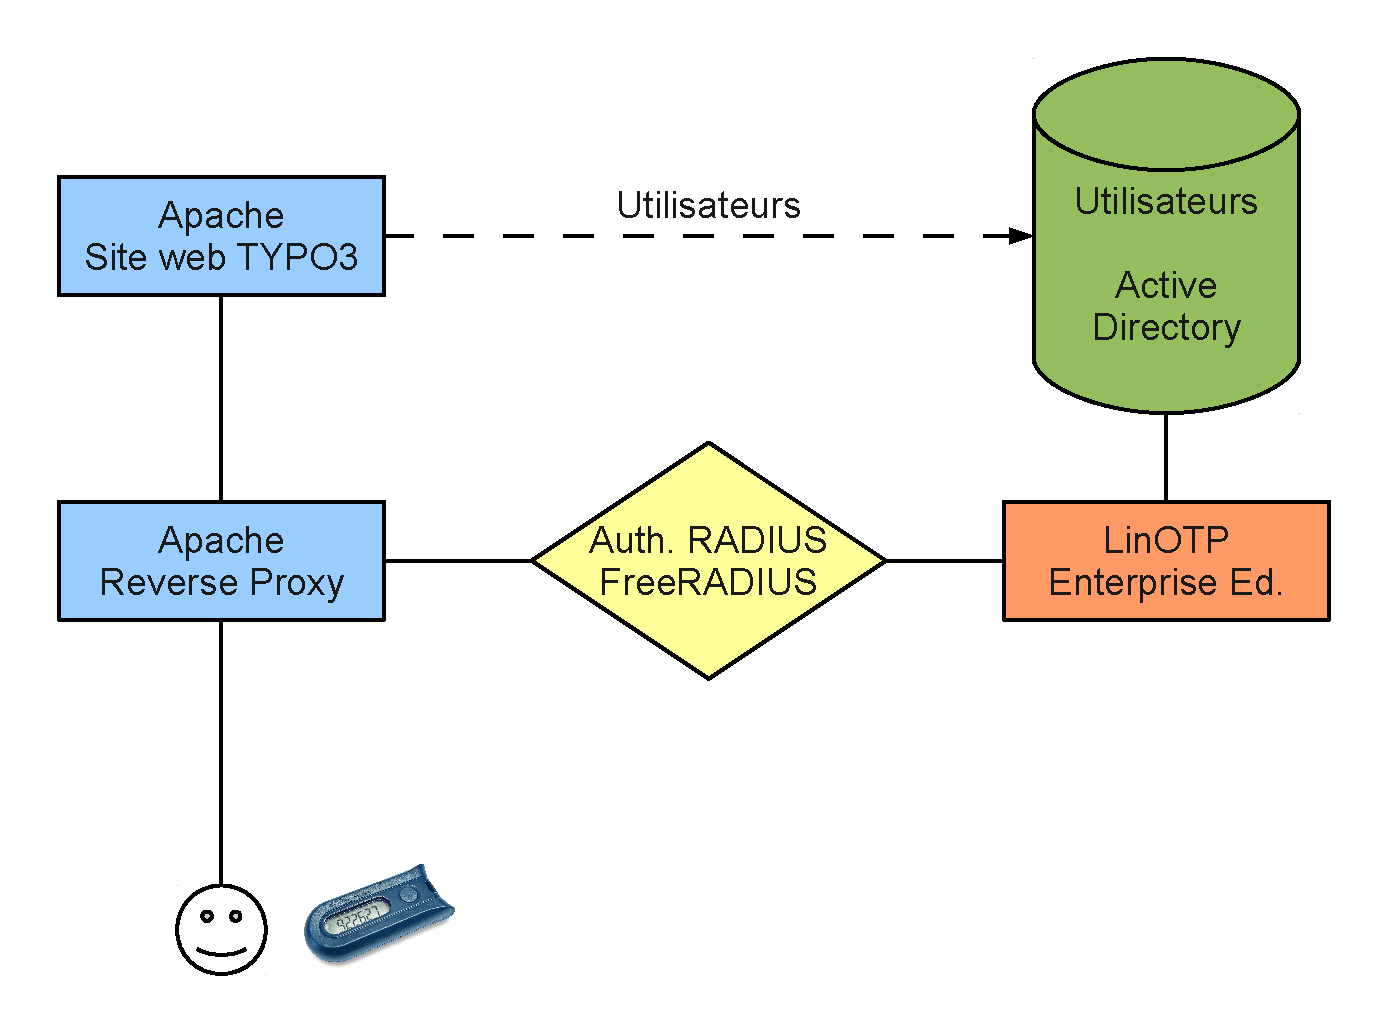
\includegraphics[width=12cm]{linotp/archi-finale}
	\caption{Architecture finale du système d'authentification OTP de la CNIL}
	\label{figure:linotp:archi-finale}
\end{figure}

\paragraph{Architecture}
L'architecture finale est illustrée en \reffigure{linotp:archi-finale}.

Le portail \aintranet{} \atypo{} reste hébergé sur son serveur Apache d'origine, qui n'est accessible que depuis le réseau interne de la CNIL.
Il conserve sa base d'utilisateurs existante qui est liée à l'annuaire \aad{}.

Un autre serveur Apache est mis en place.
Comme dans le prototype, il est configuré en tant que \arp{} pour être l'intermédiaire entre le serveur web du portail et le navigateur de l'utilisateur qui se connecte depuis \ainternet{}.
L'accès est ici aussi filtré par une authentification HTTP Basic.

Par contre, le module d'authentification pour Apache à appeler est dorénavant \amodradius{} : en tant que client \aradius{}, il se charge d'effectuer une requête sur un serveur \afreerad{}\footnote{\afreerad{} est un serveur \aradius{} libre.~\cite{freeradius}} mis en place et configuré spécialement pour ce cas d'utilisation. 
En effet, dans l'architecture finale, on a préféré une authentification via le protocole \aradius{}\footnote{\aradius{} (\etranger{Remote Authentication Dial-In User Service}) est un protocole client-serveur permettant de centraliser des données d'authentification.~\cite{radius}} plutôt que par PAM pour plusieurs raisons :

\begin{itemize}
	\item un serveur \aradius{} est indépendant du système sur lequel il est hébergé, contrairement à PAM ;
	\item le module \amodradius{} pour Apache donne un degré de configuration bien plus intéressant, en permettant entre autres de spécifier la durée de la session de l'utilisateur.
\end{itemize}

En outre, un serveur \alinotp{} Enterprise Edition est mis en place : cette version permet de supporter la connectivité avec le serveur \aradius{} et de résoudre les utilisateurs depuis l'annuaire \aad{} de la CNIL.
D'ailleurs, le serveur \afreerad{} a été compilé avec un module fourni par cette version Enterprise de \alinotp{}, ce qui permet aux deux services de communiquer entre eux.

Enfin, les utilisateurs peuvent cette fois utiliser les tokens Aladdin eToken PASS envoyés par l'éditeur \alse{} pour générer leurs OTP.

\paragraph{Intégration avec l'infrastructure du client}

\begin{figure}
	\centering
	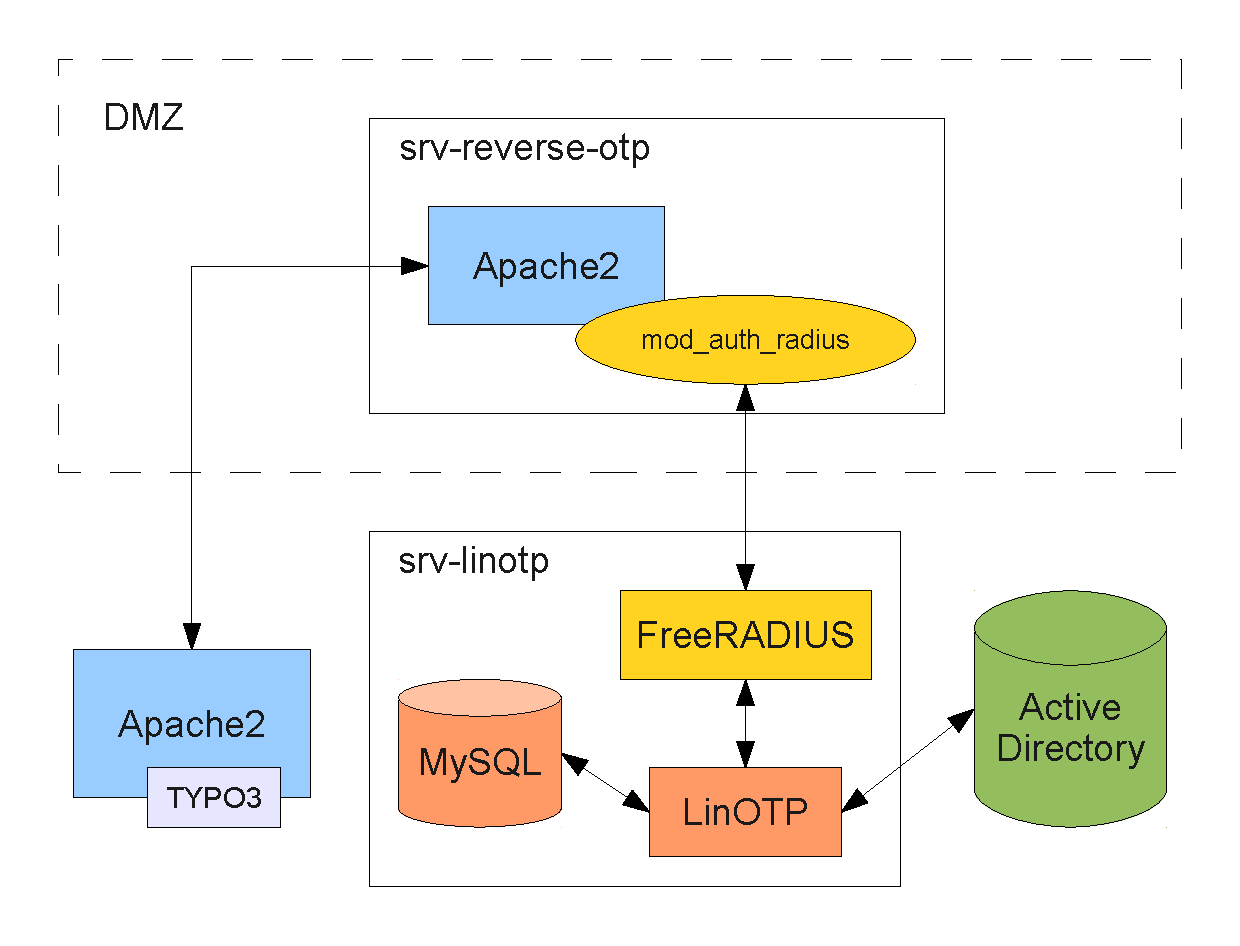
\includegraphics[width=11cm]{linotp/archi-infra}
	\caption{Intégration de la solution \alinotp{} dans l'infrastructure de la CNIL}
	\label{figure:linotp:archi-infra}
\end{figure}

Lors de la mise en place de la solution, il a fallu s'adapter et s'intégrer à l'infrastructure existante du client.
La principale contrainte technique était de monter l'architecture sur des serveurs virtualisés \alinux{} \aredhat{}.
Dans ce contexte, on a l'avantage de pouvoir utiliser autant de machines virtuelles que l'on veut car celles-ci peuvent être créées rapidement et sans coût supplémentaire significatif.

J'ai alors demandé à \amimiette{} de mettre en place deux serveurs virtualisés \aredhat{} :
\begin{itemize}
	\item le premier, \asrvotp{}, localisé dans le réseau interne et hébergeant les services \alinotp{} et \afreerad{} ;
	\item le second, \asrvrp, localisé dans une DMZ\footnote{Une zone démilitarisée (ou DMZ, de l'anglais \etranger{demilitarized zone}) est un sous-réseau isolé du réseau local par un pare-feu. Ce sous-réseau contient les machines étant susceptibles d'être accédées depuis \ainternet.~\cite{dmz}} et donc accessible depuis l'extérieur, qui héberge le \arp{}.
\end{itemize}

Ce partitionnement des services sur deux serveurs différents permet de sécuriser l'architecture.
En effet, seul le \arp{} doit être accessible de l'extérieur.
Si par exemple un pirate arrive à compromettre ce serveur web, le serveur \alinotp{} ainsi que toutes les données qui y sont relatives comme la liste des utilisateurs, les tokens qui leur sont affectés et leurs PIN correspondants ne seront pas mis en danger, à condition que la frontière entre la DMZ et le réseau interne soit suffisamment sécurisée et étanche.

Cette intégration est décrite sur la \reffigure{linotp:archi-infra}.

\paragraph{Scénario d'utilisation}

L'authentification avec un token se déroule de la façon suivante :

\begin{enumerate}
	\item l'utilisateur contacte le \arp{} depuis \ainternet{} grâce à son navigateur web ;
	\item une authentification HTTP de type Basic est demandée à l'utilisateur sur son navigateur ;
	\item l'utilisateur appuie sur le bouton du token ce qui déclenche la génération de l'OTP et son affichage sur l'écran du token ;
	\item l'OTP obtenu précédé par le PIN OTP personnel de l'utilisateur forme son mot de passe ;
	\item l'utilisateur s'authentifie dans son navigateur grâce à son identifiant et son mot de passe ;
	\item le \arp{} valide l'authentification, émet une requête HTTP vers le serveur web hébergeant le portail \atypo{} et récupère la page web demandée ;
	\item le \arp{} retourne la page web a l'utilisateur qui la visualise dans son navigateur web.
\end{enumerate}


\section{Bilan}

Cette prestation a été un succès.
En effet, le client est content du système mis en place.

Pour ma part, j'ai beaucoup appris de cette mission, tant du plan technique que relationnel.
J'ai également eu l'opportunité de me charger d'une partie de la gestion de projet en contactant divers interlocuteurs et en planifiant des rendez-vous.

